\section{Material-UI}

% @TODO: https://material.io
% @TODO: https://material.io/guidelines/
Tento framework je implementací Material Designu od společnosti Google. Material-UI obsahuje spoustu připravených komponent, které jsou na míru šité pro tvorbu aplikací díky rozsáhle studii Googlu, která je pomocí zásad a instrukcí popsaná na vlastním webu. Grafické rozhraní Aplikace je složeno z těchto komponent. Jedná se zejména o App bar, Avatar, různé varianty pro Button, Card, Dialog, Drawer, Progress, formulářové prvky, Snackbar, Tabs, ikony.

\begin{figure}[ht]
	\centering
	
\includegraphics[scale=0.5]{sections/ui/images/Appbar.png}
	\caption{Appbar}
\end{figure}

\begin{figure}[ht]
	\centering
	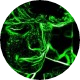
\includegraphics[scale=0.5]{sections/ui/images/Avatar.png}
	\caption{Avatar}
\end{figure}

\begin{figure}[ht]
	\mbox{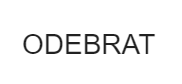
\includegraphics[scale=0.5]{sections/ui/images/Button-Flat.png}}   
	\hspace{12px}
	\mbox{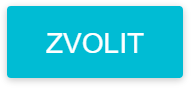
\includegraphics[scale=0.5]{sections/ui/images/Button-Raised.png}}
	\hspace{12px}
	\mbox{
\includegraphics[scale=0.5]{sections/ui/images/Button-Floating.png}}
	\hspace{12px}
	\mbox{
\includegraphics[scale=0.5]{sections/ui/images/Button-Icon.png}}
	\caption[Button]{Flat, Raised, Floating Action a Icon Button}
\end{figure}

\begin{figure}[ht]
	\centering
	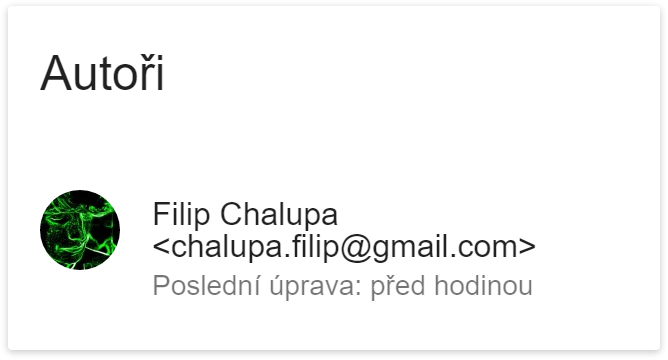
\includegraphics[scale=0.5]{sections/ui/images/Card.png}
	\caption[Card]{Card, rámeček sloužící k seskupení souvisejícího obsahu}
\end{figure}

\begin{figure}[ht]
	\centering
	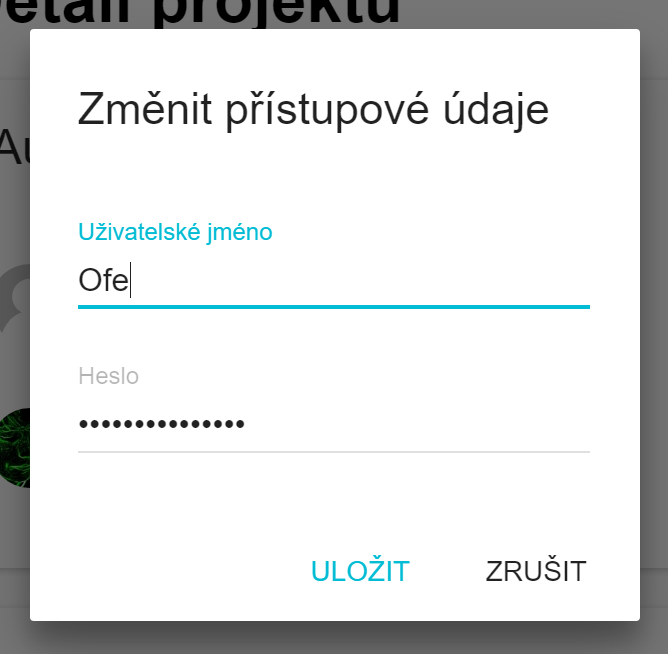
\includegraphics[scale=0.5]{sections/ui/images/Dialog.png}
	\caption[Dialog]{Dialog zobrazuje modální okna uvnitř aplikace}
\end{figure}

\begin{figure}[ht]
	\centering
	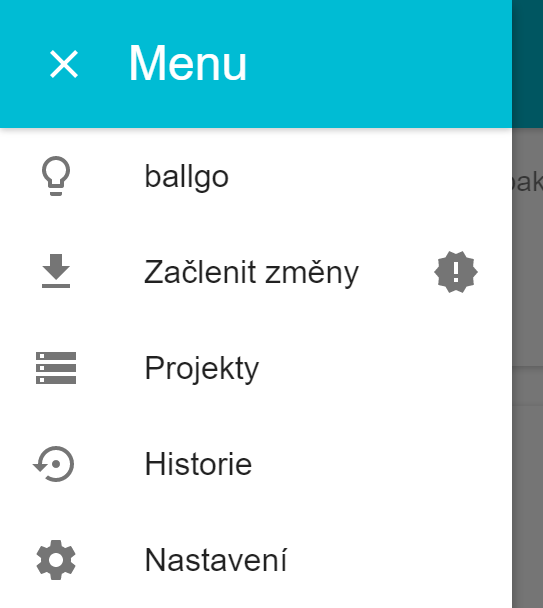
\includegraphics[scale=0.5]{sections/ui/images/Drawer.png}
	\caption[Drawer]{Drawer, boční vysouvací nabídka}
\end{figure}

\FloatBarrier

Progress, znázornění právě probíhající akce. Například načítání historie projektu.

Text Field pro psaní textu, Checkbox a Toggle pro zaškrtávání či povolení a zakázání.

Snackbar, informační lišta o právě proběhlé akci.

Tabs, skrytí osahu.

Ikony

% @TODO: ikony https://material.io/icons/
